\section{XFS Performance As Backend File System}

Ceph supports multiple backend file systems including Btrfs, Ext4, and XFS.
Due to its maturity and Inktank's recommendations, we chose XFS.\footnote{It
should be noted that in testing cases while we can compare XFS vs.
Brtfs, Brtfs generally shows better performance results.} We experimented with
XFS to acquire a set of configuration parameters which provided optimal
performance for the SFA10K. We sampled a selected set of parameters (block size,
queue depth, request size, sequential read and write). We settled on the
following configuration: mount with \verb!nobarrier,noatim,inode64! options.
The \verb!inode64! option had a notable improvement on sequential write (around
20\%).

%% Can the graphs be adjusted to have the same values in the Y axis?
\begin{figure}[htb]
\centering
%% -- 1st figure
\centering
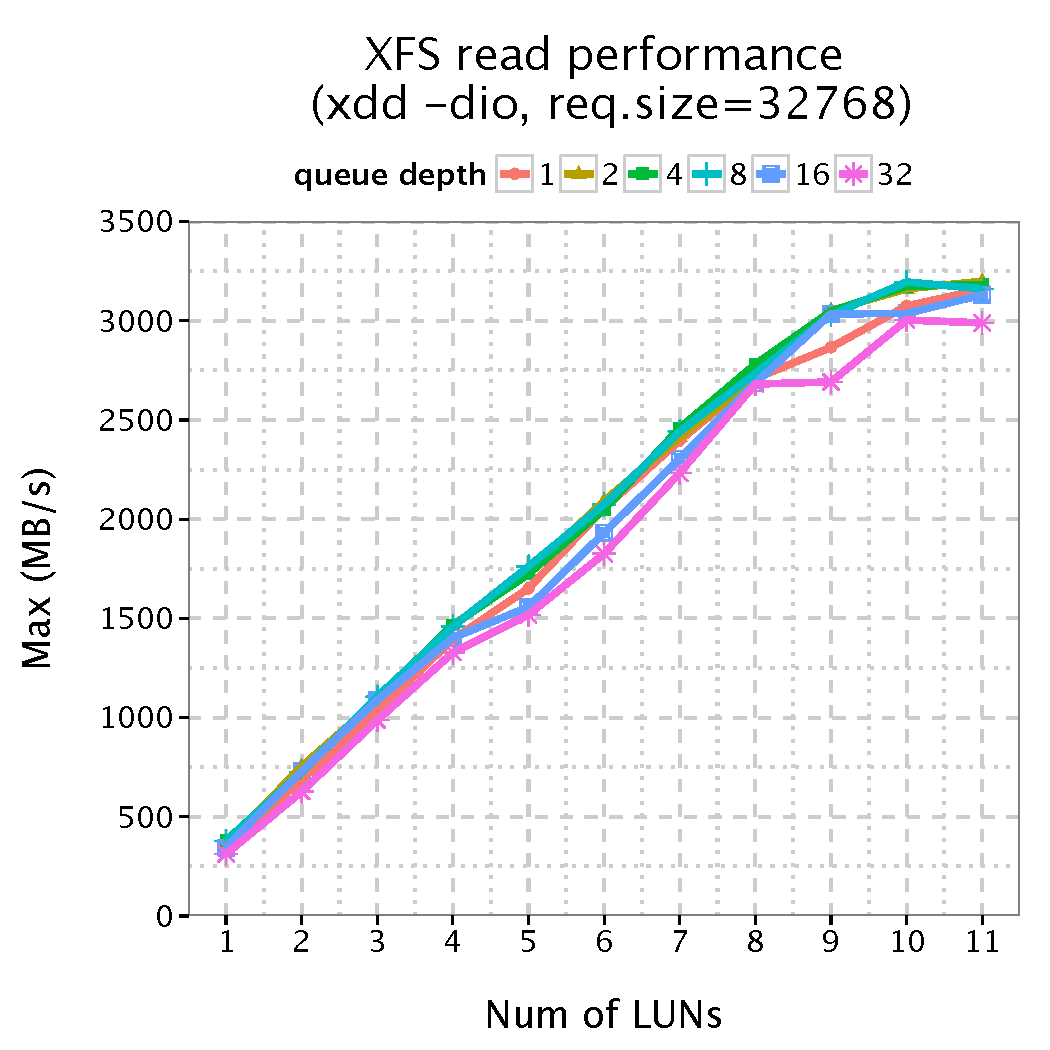
\includegraphics[width=3in]{data/xdd-read}
\caption{XFS read performance scaling on number of devices}
\label{fig:xfs-read}
\end{figure}

\begin{figure}[htb]
\centering
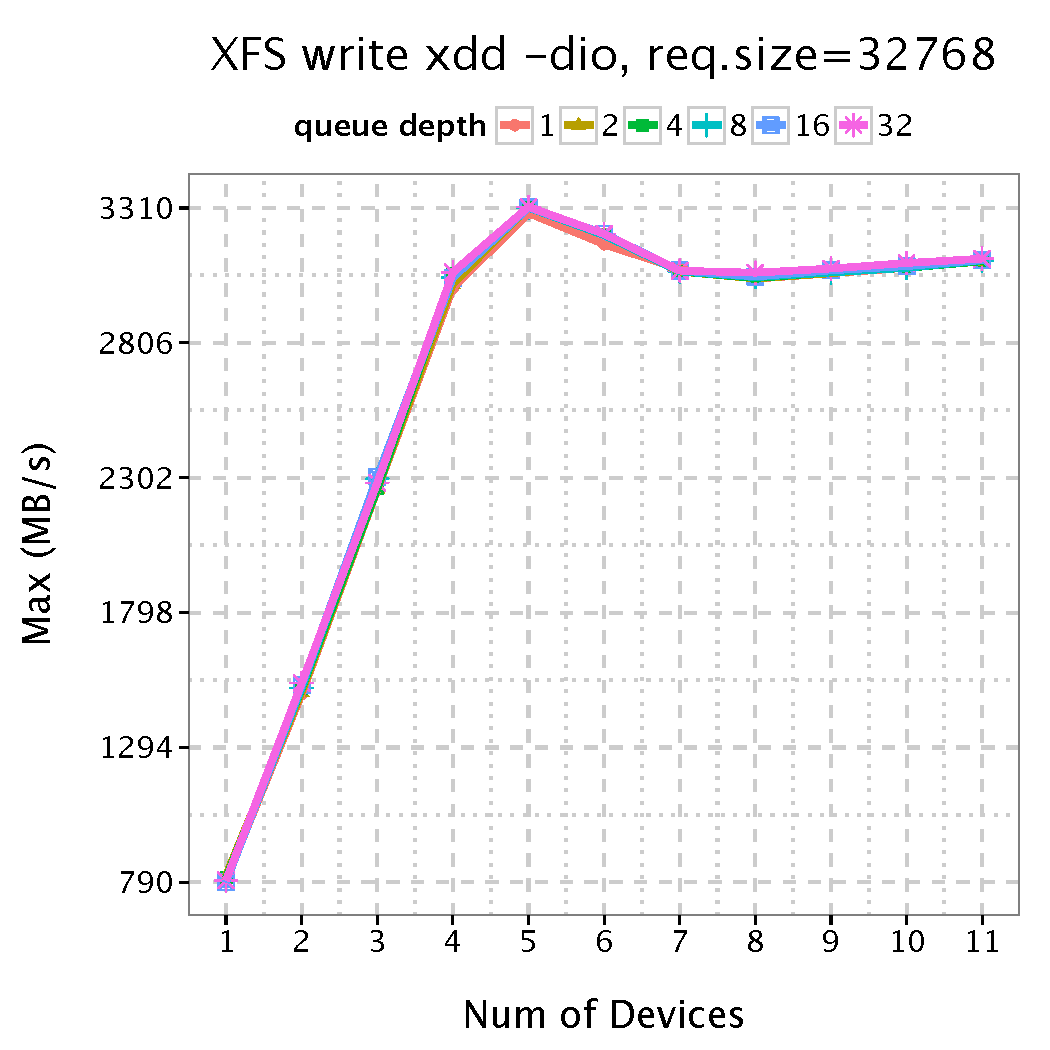
\includegraphics[width=3in]{data/xdd-write}
\caption{XFS write performance scaling on number of devices}
\label{fig:xfs-write}
\end{figure}



%\begin{figure}[htb]
%\centering
%% -- 1st figure
%\begin{minipage}[t]{0.5\linewidth}
%\centering
%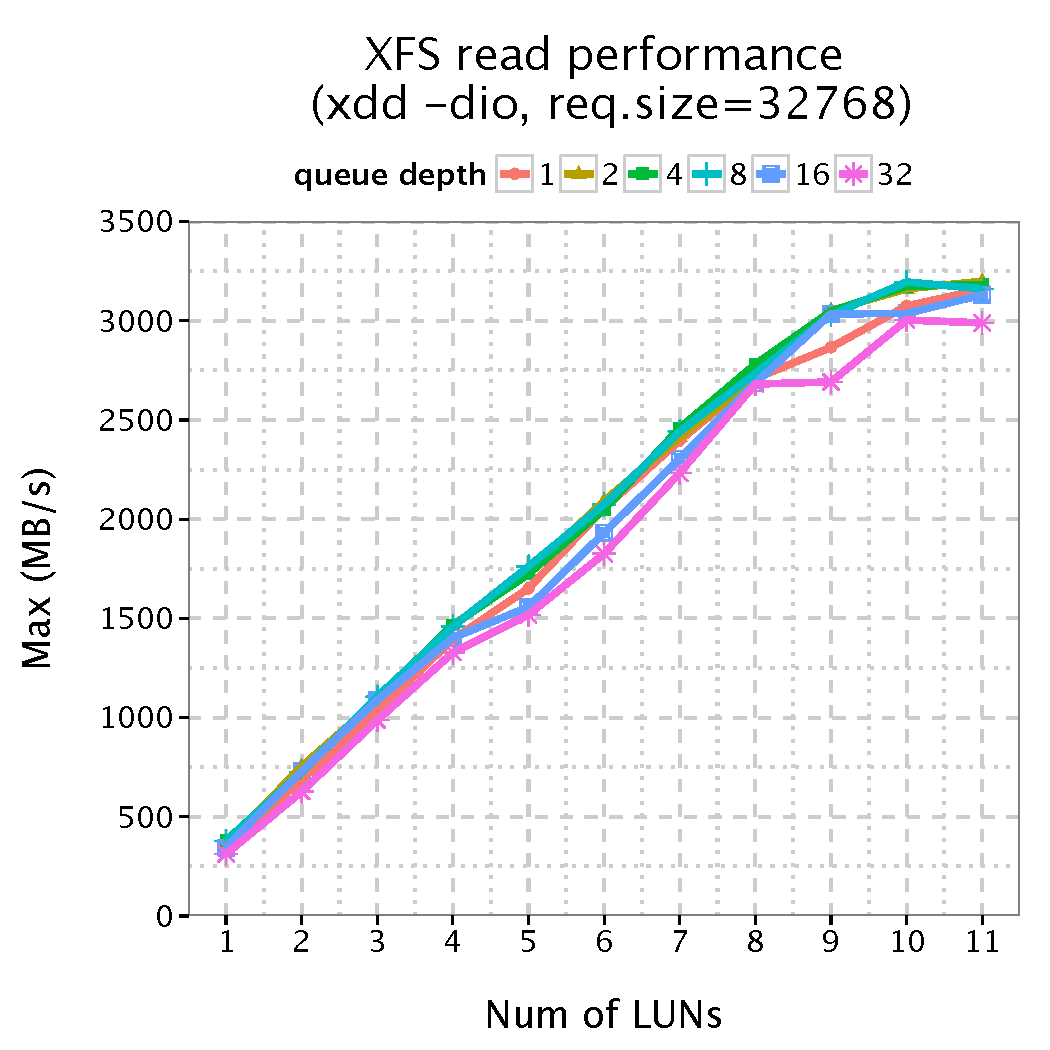
\includegraphics[width=3in]{data/xdd-read}
%\caption{XFS read performance scaling on number of devices}
%\label{fig:xfs-read}
%\end{minipage}%
%\begin{minipage}[t]{0.5\linewidth}
%\centering
%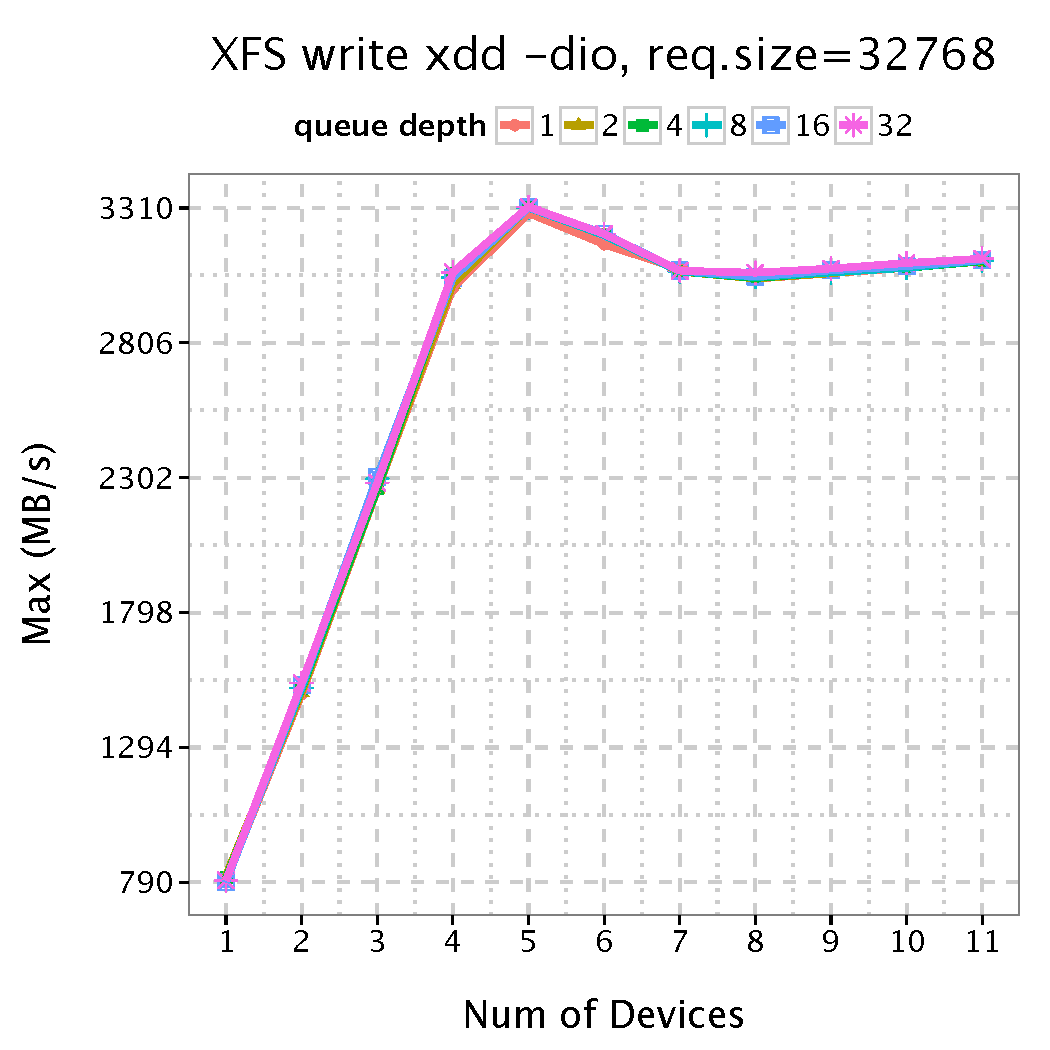
\includegraphics[width=3in]{data/xdd-write}
%\caption{XFS write performance scaling on number of devices}
%\label{fig:xfs-write}
%\end{minipage}%
%\end{figure}



% % Are the read and write graphs wrong or should the second sentence below be
% about write % instead of read?

The read and write performance results are summarized in
Figures~\ref{fig:xfs-read} and~\ref{fig:xfs-write}, respectively. These graphs
show scaling behavior over the number of LUNs, which indicates that XFS can
reach the peak write performance with just five SATA LUNs. Increasing number
of LUNs beyond 5, degradation happened.  Also, we did not observe any obvious
differences in performance when varying the queue depth parameter.  For these
tests, we used the \verb!xdd! benchmark with direct I/O and a request size of
32 KB.

